\documentclass[12pt, a4papre]{article}
\usepackage[catalan]{babel}
\usepackage[unicode]{hyperref}
\usepackage{amsmath}
\usepackage{amssymb}
\usepackage{amsthm}
\usepackage{xifthen}
\usepackage{siunitx}
\usepackage{xcolor}
\usepackage{float}
\usepackage[utf8]{inputenc}

\usepackage{listings}
\usepackage{setspace}
\usepackage{graphicx}
\usepackage{tikz,lipsum,lmodern}
\usepackage[most]{tcolorbox}
\usepackage{circuitikz}
\usepackage{indentfirst}
\usepackage{verbatimbox}
\definecolor{mygreen}{RGB}{28,172,0} % color values Red, Green, Blue
\definecolor{mylilas}{RGB}{170,55,241}
\usepackage{listings}
\lstdefinelanguage{vhdl}{
   morekeywords={
     library,use,all,entity,is,port,in,out,end,architecture,of,
     begin,and
   },
   morecomment=[l]--
}
\usepackage{xcolor}
\colorlet{keyword}{blue!100!black!80}
\colorlet{comment}{green!50!black!90}
\lstdefinestyle{vhdl}{
   language     = VHDL,
   basicstyle   = \ttfamily,
   keywordstyle = \color{keyword}\bfseries,
   commentstyle = \color{comment}
}

\graphicspath{ {./Imatges/} }


\newcommand{\norm}[1]{\lvert #1 \rvert}

\hypersetup{
    colorlinks = true,
    linkcolor = blue
}

\author{Daniel Vilardell\\
	   Igor Yuziv}
\title{\textbf{Memoria Practica 2}}
\date{}

\begin{document}
	\maketitle
	\tableofcontents
     
     \newpage

	\section{Diseny Jerarquic}
	
	El diseny te l'objectiu de multiplicar dos nombres compresos entre 0 i 9 entrats desde la graella de la placa. Nomes es podra entrar dades quan el estat intro estigui activat i nomes es veurà el resultat quan estiguem en el estat show. El estat intro s'activa clicant al boto asterisc mentres que el estat show s'activa si es clica el botó coixinet. 
	
	El diseny principal \textbf{ppal} el que fa es rebre la tecla premuda i el bloc keygroup ens diu si es un coixinet, un asterisc o un nombre. Control rebra aquesta informacio i decidirà si mostra o no el resultat en funcio del estat que esta. També decidirà si deixa entrar dades o no, i en el cas que si, la sortida intro sera 1 i el bloc regs actualitzara el nombre amb el rebut per la tecla. Finalment els valors de opA i opB guardats es multipliquen i si estem en el estat de show es mostra el resultat, i si no no es mostra.
	
	El diseny exterior, que te la finalitat de comunicar el programa principal amb la placa desde la que introduim les dades funciona de la seguent manera. Es llegeixen les dades i s'introdueix la informacio que ens donen els blogs keytest i f\_div a ppal(si sha premut alguna tecla, quina sha premut, si sha de resetejar el sistema i el rellotge). El component ppal extreu opA, opB i el resultat del producte junt amb el bit de show, que ens dirà si mostrem el resultat i els leds vermells o no el mostrem i iluminem els leds verds.
	
	El següent dibuix mostra un diagrama intuitiu del funcionament del sistema.
	
	\begin{figure}[H]
		\begin{center}
		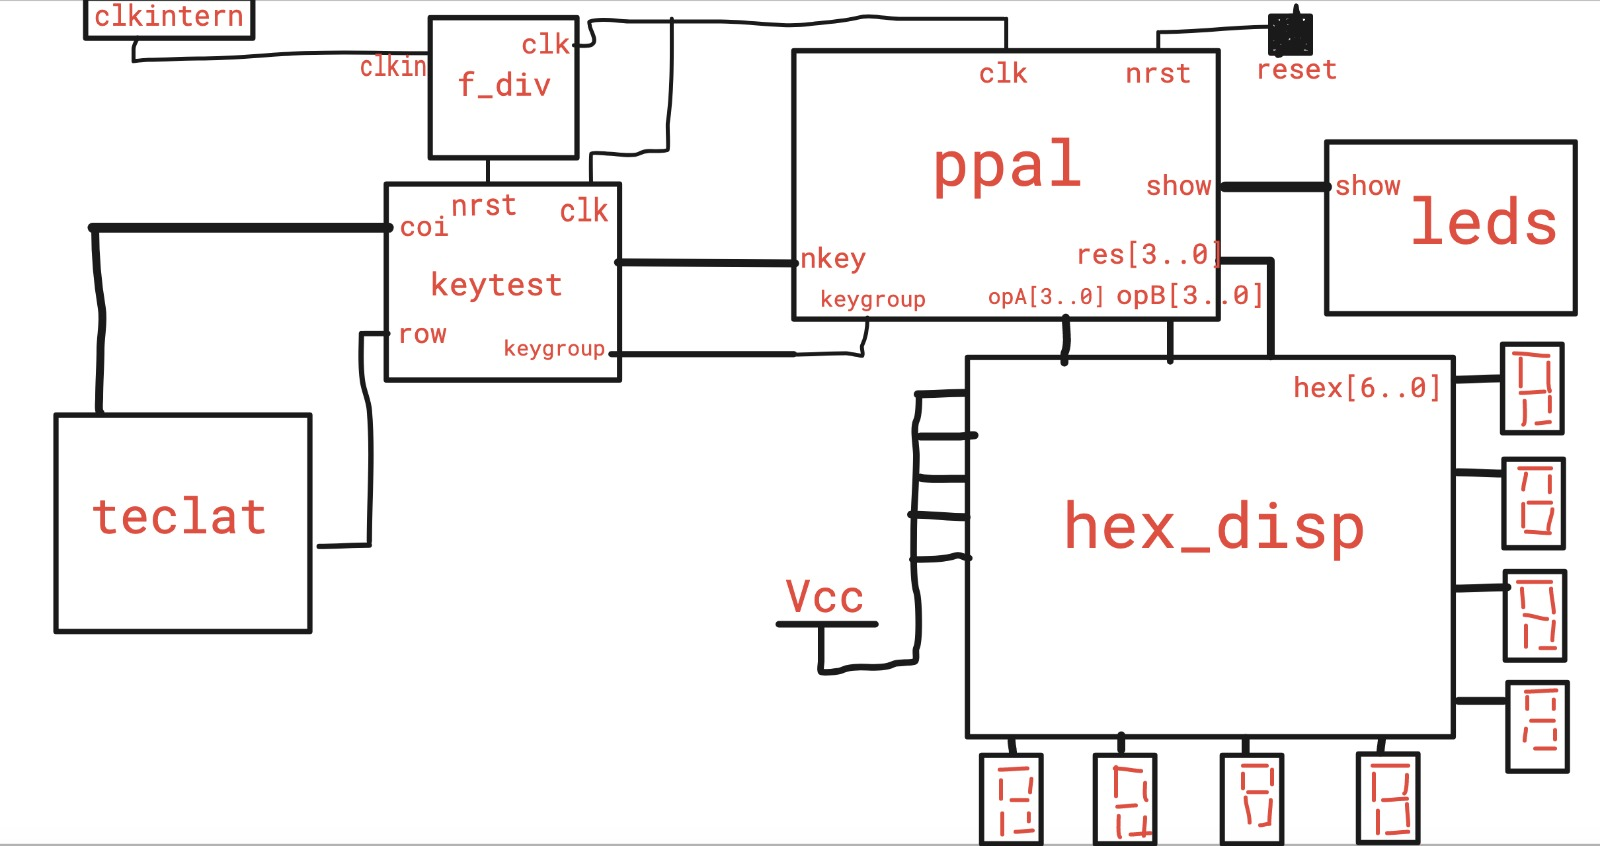
\includegraphics[width=130mm]{Dibuix_diseny.jpeg}
		\end{center}
	\end{figure}
	
	\newpage
	\section{Blocs}
	
	\subsection{Conversor binari a BCD de 8 bits}
	
	Aquest component el farem amb vhdl i te l'objectiu de convertir la sortida del multiplicador de 8 bits a bcd per tal de mostrar a la placa. Te la seguent forma
	\begin{lstlisting}[style=vhdl, frame=single, basicstyle=\tiny]
LIBRARY ieee; USE ieee.std_logic_1164.ALL;  

ENTITY BIN_BCD_8B IS PORT (   
	BIN : IN STD_LOGIC_VECTOR(7 downto 0);   
	BCD : OUT STD_LOGIC_VECTOR(7 downto 0)); 
END BIN_BCD_8B;  

ARCHITECTURE taula_veritat OF BIN_BCD_8B IS   
	BEGIN 
	with BIN SELECT BCD <=     	
		"10011001" WHEN "00111000",  -- 81     
		"01110010" WHEN "01001000",  -- 72      
		"01100100" WHEN "01000000",  -- 64     
		"01010110" WHEN "00111000",  -- 56     
		"01010100" WHEN "00111000",  -- 54        
		"01001001" WHEN "00110001",  -- 49     
		"01001000" WHEN "00110000",  -- 48     
		"01000101" WHEN "00101101",  -- 45     
				.
				.
				. 
		"--------" WHEN OTHERS;   
END taula_veritat;
\end{lstlisting}

\begin{figure}[H]
		\begin{center}
		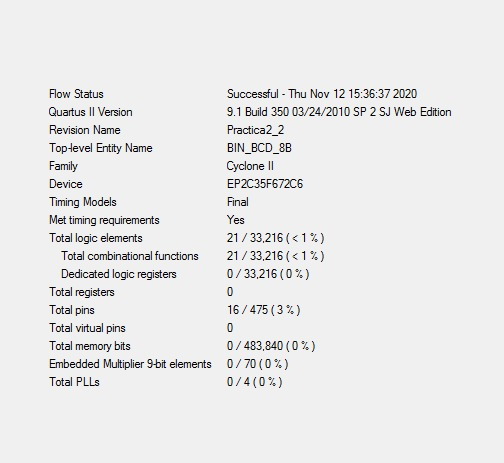
\includegraphics[width=130mm]{informeBIN_BCD_8B.jpeg}
		\end{center}
	\end{figure}


	\begin{table}[h!]
		\centering
		 \begin{tabular}{|c | c|} 
			 \hline
			 Entrades & Descripció\\ [0.5ex] 
			 \hline
			 BIN(8) &  Nombre en binari que es vol convertir a BCD\\ 
			 \hline\hline
			 Sortides & Descripció\\ [0.5ex] 
			 \hline
			 BCD(8) & Nombre BIN convertit a BCD\\ 
			 \hline
		 \end{tabular}
	\end{table}
	
	\begin{figure}[H]
		\begin{center}ño 
		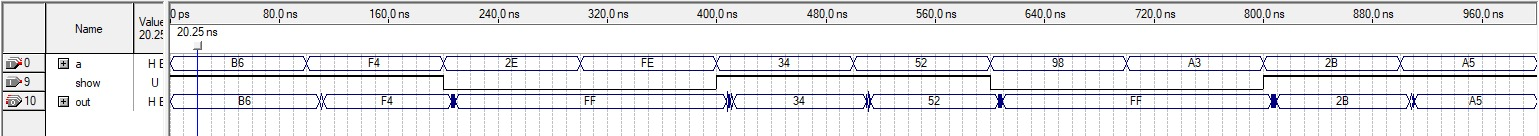
\includegraphics[width=130mm]{selSimulacio.jpeg}
		\end{center}
	\end{figure}
	
	Podem veure que la simulacio funciona ja que la entrada en binari es igual que la sortida en hexadecimal, es a dir, en BCD.
	
	\subsection{Conversor de binari de 4 bits a 8 bits}
	
	Aquest component el conectarem abans de la entrada del multiplicador per a transformar la entrada de 4 bits a la que necessita el multiplicador que es de 8 bits. Aquest l'unic que farà es omplir de 0 les primeres 4 entrades.
	\begin{figure}[H]
		\begin{center}
		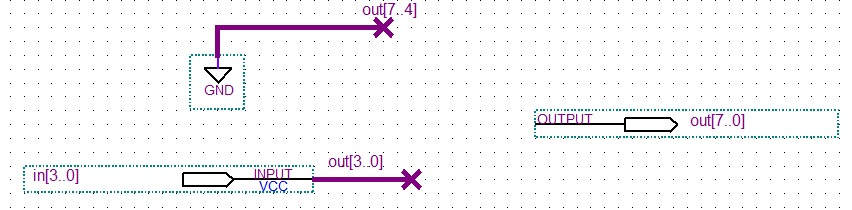
\includegraphics[width=130mm]{Bin_4_8.jpeg}
		\end{center}
	\end{figure}
	
	\begin{figure}[H]
		\begin{center}
		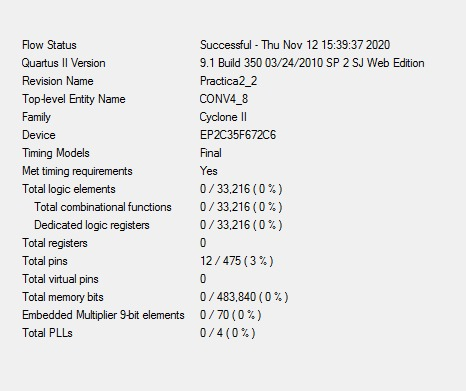
\includegraphics[width=130mm]{informeCONV4_8.jpeg}
		\end{center}
	\end{figure}
	
	\begin{table}[h!]
		\centering
		 \begin{tabular}{|c | c|} 
			 \hline
			 Entrades & Descripció\\ [0.5ex] 
			 \hline
			 in(4) &  Nombre de 4 bits\\ 
			 \hline\hline
			 Sortides & Descripció\\ [0.5ex] 
			 \hline
			 out(8) & Sortida de 8 bits\\ 
			 \hline
		 \end{tabular}
	\end{table}
	
	\begin{figure}[H]
		\begin{center}
		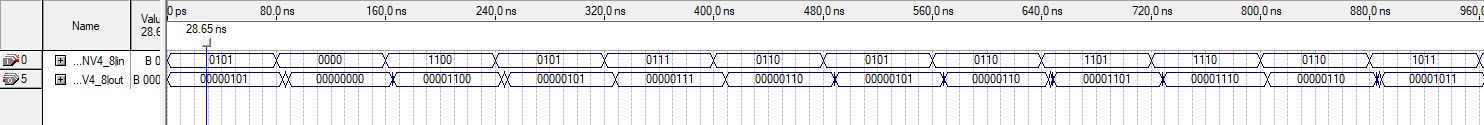
\includegraphics[width=130mm]{4_8Simulacio.jpeg}
		\end{center}
	\end{figure}
	
	Podem veure que el component funciona a partir de la simulació ja que els nombres son els mateixos que els de la sortida pero la sortida te 8 bits en contes de 4.
	
	\subsection{Keygroup}
	
	Aquest component ens dirà si la tecla premuda es el asterisc(AST), el coixinet(COI) o el nombre en BCD. A mes comproba abans que s'estigui prement alguna tecla amb la entrada nkey. Això ho fem amb el diseny comentat al previ que té la seguent forma.
	
	\begin{figure}[H]
		\begin{center}
		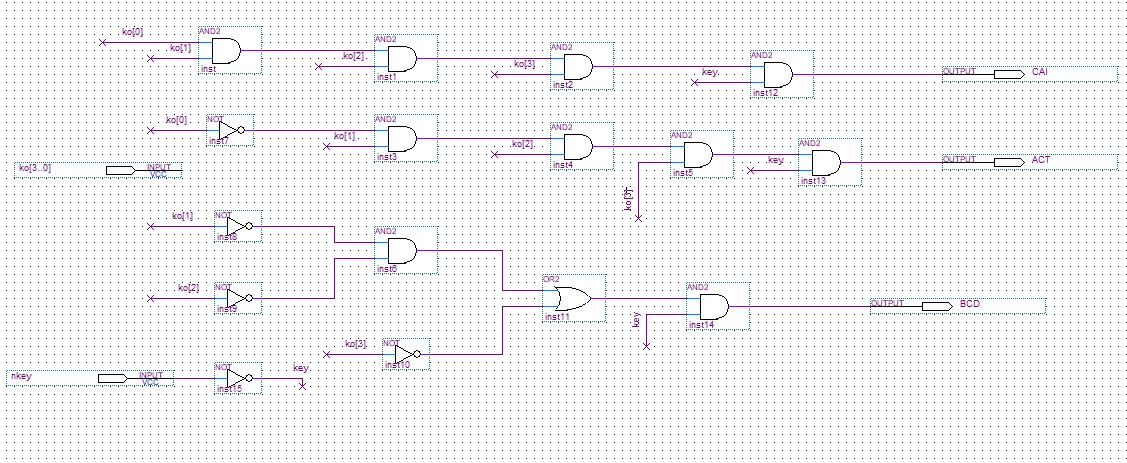
\includegraphics[width=130mm]{Keycode.jpeg}
		\end{center}
	\end{figure}
	\begin{figure}[H]
		\begin{center}
		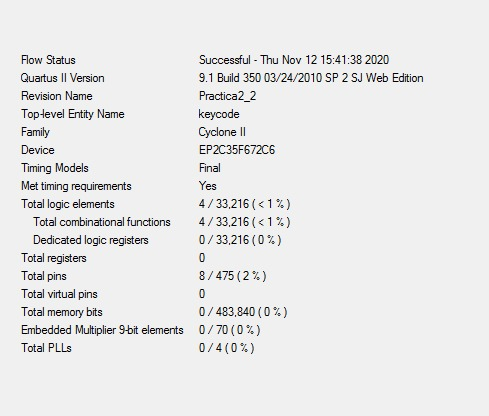
\includegraphics[width=130mm]{informekeygroup.jpeg}
		\end{center}
	\end{figure}
	
	\begin{figure}[H]
		\begin{center}
		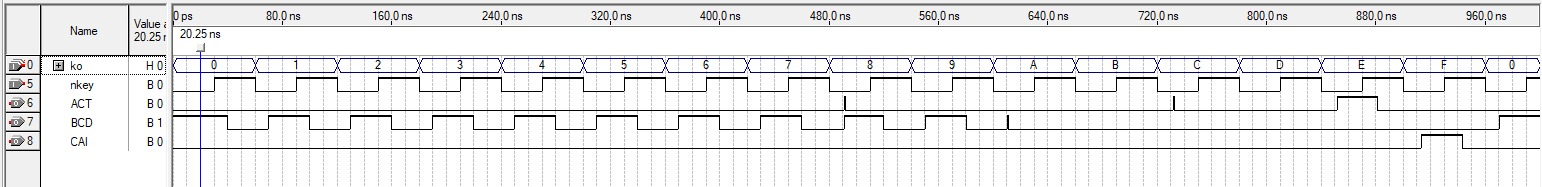
\includegraphics[width=130mm]{KCsim.jpeg}
		\end{center}
	\end{figure}
	
	Podem veure que la simulació mostra el correcte funcionament ja que desde la entrada 0 fins a la 9 informa que la entrada keycode es un nombre, de la A fins a la D els tres estan a 0, la entrada E diu que es un asterisc i la entrada F que es un coixinet.
	
	La descripció del bloc en VHDL es la següent.
	
		\begin{lstlisting}[style=vhdl, frame=single, basicstyle=\tiny]
library ieee;
use ieee.std_logic_1164.all;

entity keygroup_v is
	port(nkey : in std_logic;
		k : in std_logic_vector(3 downto 0);
		bcd, ast, coi : out std_logic);
end keygroup_v;

architecture arq of keygroup_v is
begin
process (nkey, k)
begin
	if (nkey = '0' and (k = "0000" or k = "0001" or k = "0010" or
				   k = "0011" or k = "0100" or k = "0101" or
				   k = "0110" or k = "0111" or k = "1000" or
				   k = "1001")) then bcd <= '1'; ast <= '0'; coi <= '0';
	elsif(nkey = '0' and k = "1110")
			then bcd <= '0'; ast <= '1'; coi <= '0';
	elsif(nkey = '0' and k = "1111")
			then bcd <= '0'; ast <= '0'; coi <= '1';
	else bcd <= '0'; coi <= '0'; ast <= '0';
	end if;
end process;

end arq;
\end{lstlisting}
	
	\subsection{Multiplicador}
	
	Aquest component t'he l'objectiu de multiplicar 2 nombres de 4 bits i treure la sortida en BCD de 4 bits, es a dir, 8 bits de sortida. Per a fer això usarem el component creat a la practica anterior que et multiplicava dos nombres de 8 bits. A la entrada hi posarem un conversor de 4 a 8 bits i a la sortida un conversor de binari de 8 bits a BCD que crearem amb vhdl.
	
	\begin{figure}[H]
		\begin{center}
		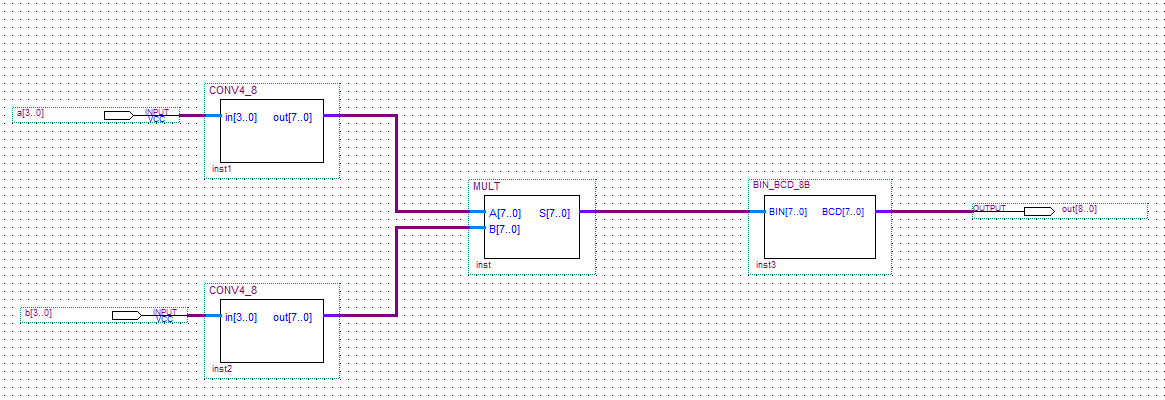
\includegraphics[width=130mm]{Mult_Bin_BCD.jpeg}
		\end{center}
	\end{figure}
	
	\begin{figure}[H]
		\begin{center}
		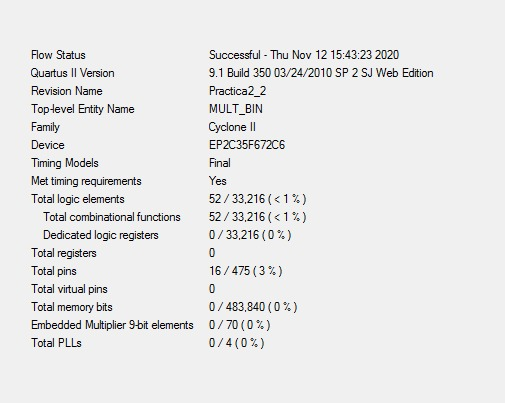
\includegraphics[width=130mm]{informeMULT.jpeg}
		\end{center}
	\end{figure}
	
	\begin{table}[h!]
		\centering
		 \begin{tabular}{|c | c|} 
			 \hline
			 Entrades & Descripció\\ [0.5ex] 
			 \hline
			 a(4) &  Nombre a de 4 bits que es vol multiplicar\\ 
			 b(4) &  Nombre b de 4 bits que es vol multiplicar\\ 
			 \hline\hline
			 Sortides & Descripció\\ [0.5ex] 
			 \hline
			out (8) & Sortida de 8 bits amb el resultat de la multiplicació\\ 
			 \hline
		 \end{tabular}
	\end{table}
	
	\begin{figure}[H]
		\begin{center}
		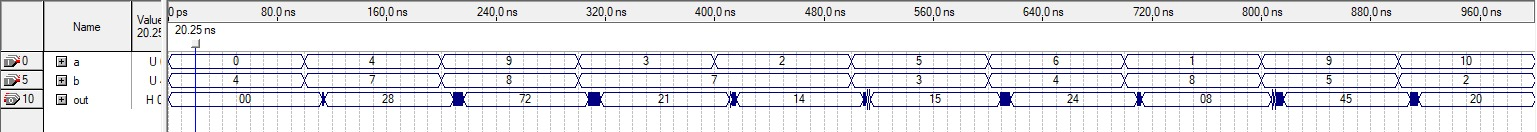
\includegraphics[width=130mm]{SimMult.jpeg}
		\end{center}
	\end{figure}
	
	Podem veure que funciona a partir de la simulacio ja que retorna la multiplicacio de a i b en BCD ja que representem la solucio en hexadecimal.
	
	La descripció del bloc en VHDL es la següent.
	
	\begin{lstlisting}[style=vhdl, frame=single, basicstyle=\small]
library ieee;
use ieee.std_logic_1164.all;
USE IEEE.NUMERIC_STD.ALL;

entity AperB_v is
	port(a, b : in std_logic_vector(3 downto 0);
		  z : out std_logic_vector(7 downto 0));
end AperB_v;

architecture arq of AperB_v is
begin
	z <= std_logic_vector(unsigned(a)*unsigned(b));
end arq;
\end{lstlisting}
	
	\subsection{Bloc sel}
	
	Aquest bloc te l'objectiu de retornar un bus de 7 bits amb el nombre $a$ si la entrada $show$ es 1, i 1111111 si la entrada $show$ es 0;
	\begin{figure}[H]
		\begin{center}
		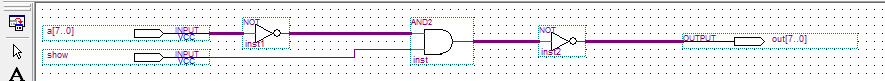
\includegraphics[width=130mm]{SEL.jpeg}
		\end{center}
	\end{figure}
	
	\begin{figure}[H]
		\begin{center}
		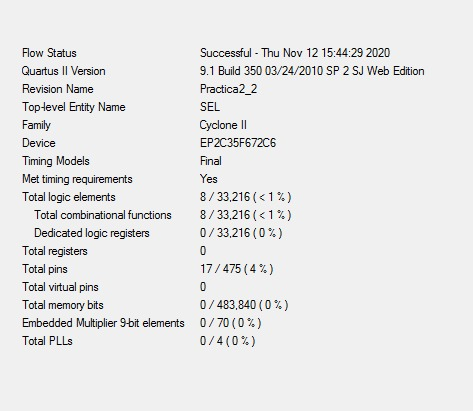
\includegraphics[width=130mm]{informeSEL.jpeg}
		\end{center}
	\end{figure}
	
	\begin{table}[h!]
		\centering
		 \begin{tabular}{|c | c|} 
			 \hline
			 Entrades & Descripció\\ [0.5ex] 
			 \hline
			 a(8) &  Nombre a seleccionar\\ 
			 show(1) &  Nombre que decideix si la sortida es a o 11111111\\ 
			 \hline\hline
			 Sortides & Descripció\\ [0.5ex] 
			 \hline
			out (8) & Sortida de 8 bits amb el resultat de la multiplicació\\ 
			 \hline
		 \end{tabular}
	\end{table}
	
	\begin{figure}[H]
		\begin{center}
		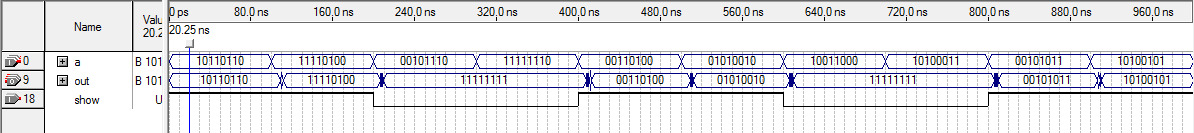
\includegraphics[width=130mm]{Simulacio_Sel.jpeg}
		\end{center}
	\end{figure}
	
	Podem veure que la simulacio funciona ja que si sel es 0 la sortida es 11111111 i si sel es 1 la sortida es a(8).
	
	La descripció del bloc en VHDL es la següent.
	
	\begin{lstlisting}[style=vhdl, frame=single, basicstyle=\small]
LIBRARY ieee ; 
USE ieee.std_logic_1164.ALL;

ENTITY sel_v IS PORT (
	a  :  IN STD_LOGIC_VECTOR(7  downto  0 );
	show : IN STD_LOGIC;
	o : OUT STD_LOGIC_VECTOR(7  downto  0 ) ) ;
END sel_v

;ARCHITECTURE arq OF sel_v IS
begin
process(show)
BEGIN
	if(show = '1') then o <= a;
	else o <= "11111111";
	end if;
END process ;
END arq;
\end{lstlisting}
	
	\subsection{Regs}
	
	Aquest component es un mòdul seqüencial síncron que te com a finalitat carregar i memoritzar els operands de la multiplicació opA i opB. Aquest, si la entrada intro es 1 i clk esta en el flanc de pujada i nrst esta activat, actualitzara els valors de opA i opB, posant a opA el valor entrat per keycode i a opB el antic valor de opA.
	
	\begin{figure}[H]
		\begin{center}
		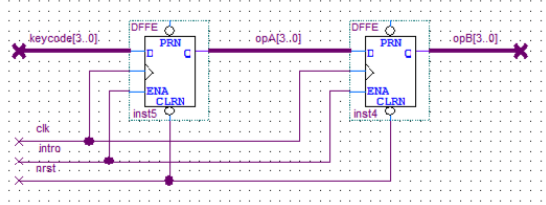
\includegraphics[width=130mm]{regs.png}
		\end{center}
	\end{figure}
	
	\begin{figure}[H]
		\begin{center}
		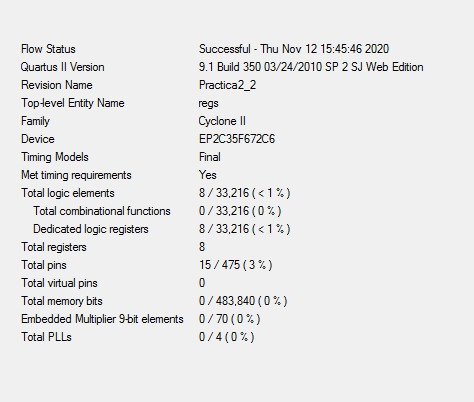
\includegraphics[width=130mm]{informeREGS.jpeg}
		\end{center}
	\end{figure}
	
	\begin{table}[h!]
		\centering
		 \begin{tabular}{|c | c|} 
			 \hline
			 Entrades & Descripció\\ [0.5ex] 
			 \hline
			 keycode(4) & Marca la tecla que s'està prement \\
			 clk(1) & Es el rellotge que gestionara la memoria del sistema\\
			 intro(1) & Indica si s'esta entrant un numero i s'ha d'actualitzar\\
			 nrst(1) & Marcara si s'ha de resetejar a 0 o no \\ [1ex] 
			 \hline\hline
			 Sortides & Descripció\\ [0.5ex] 
			 \hline
			 opA(8) & El valor del nombre A guardat\\
			 opB(8) & El valor del nombre B guardat\\
			 \hline
		 \end{tabular}
	\end{table}
	
	\begin{figure}[H]
		\begin{center}
		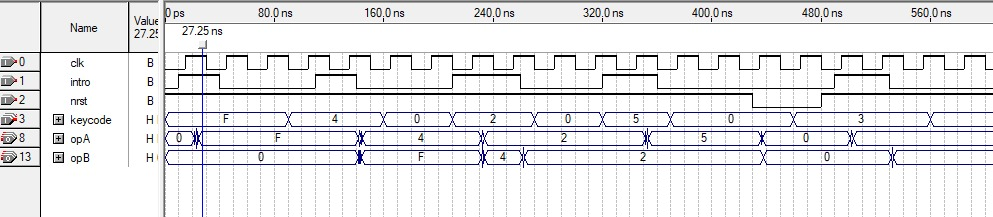
\includegraphics[width=130mm]{SimRegs.jpeg}
		\end{center}
	\end{figure}
	
	Per a veure que el bloc funciona estem simulant la seguent situació. Primer es prem la tecla asterisc per tal d'introduir dades i despres s'introdueix un valor numeric 4 que es guarda en la variable opA. Despres s'introdueix un altre valor numeric 2 que fa que el 4 es guardi a opB i el 2 a opA. Al introduir el tercer valor aquest es posa a opA, el de opA passa a opB i el de opB desapareix. Mes tard premem el boto de reset que posa els dos valors a 0.
	
	La descripció del bloc en VHDL es la següent.
	
	\begin{lstlisting}[style=vhdl, frame=single, basicstyle=\tiny]
library ieee;
use ieee.std_logic_1164.all;

entity regs_v is
	port(clk, nrst, intro : in std_logic;
		 keycode : in std_logic_vector(3 downto 0);
		 opA, opB: out std_logic_vector(3 downto 0));
end regs_v;

architecture arq of regs_v is
signal a, b : std_logic_vector(3 downto 0);
begin
process (clk, nrst)
begin 
	if(nrst = '0') then a <= "0000"; b <= "0000";
	elsif(nrst='1') and (clk'event and clk = '1') and (intro = '1') then
			b <= a;
			a <= keycode;
	end if;
end process;
opA <= a;
opB <= b;

end arq;
\end{lstlisting}
	
	\subsection{Control}
	
	Aquest component ens ve donat i esta escrit en vhdl. L'objectiu es guardar el estat en el que estem i indicar als altres moduls si es poden introduir nombres e iluminar els leds verds o mostrar el resultat i iluminar els leds vermells. En el cas que es premi coixinet el estat passarà a ser show, mentres que si es prem asterisc sera intro. Si es prem un nombre el estat es mantindra, i si estem en estat intro, enviara la senyal per a actualitzar els valors de opA i opB. Si estem en estat show no passara res.
	
	\begin{figure}[H]
		\begin{center}
		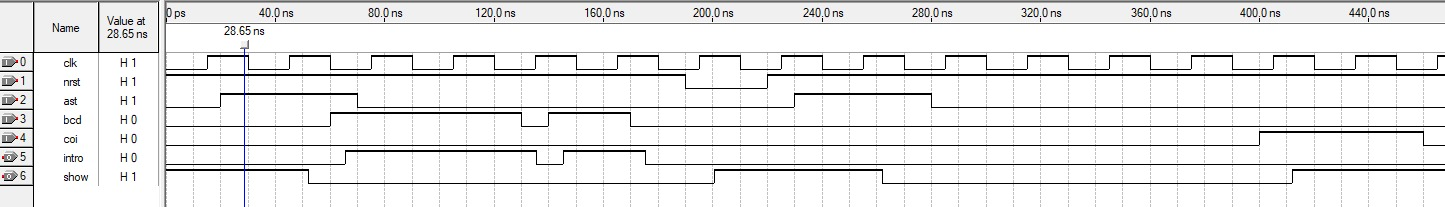
\includegraphics[width=130mm]{SimControl.jpeg}
		\end{center}
	\end{figure}
	
	La simulacio del component ens mostra que es correcte ja que quan es clica asterisc es passa en el estat st\_intro, en el que si cliquem un valor numeric el bit intro s'activa i el bit show esta desactivat. Quan cliquem coixinet podem veure al final que s'activa el bit de show. Quan cliquem reset es posa en el estat inicial que te show activat.
	
	
	\subsection{Leds}
	
	Aquest component encendrà els leds vermells quan no es puguin introduir nombres i els verds quan si que es puguin introduir. Això es decidirà en funció de la entrada show.
	
		\begin{lstlisting}[style=vhdl, frame=single, basicstyle=\small]
library ieee;
use ieee.std_logic_1164.all;

entity LEDS is 
	port( show : in std_logic;
	LEDV, LEDG: out std_logic_vector (3 downto 0));
end LEDS;

architecture arq of LEDS is
begin
process (show) begin
if (show = '0') then
	LEDV <= "0000";
	LEDG <= "1111";
else
	LEDG <= "0000";
	LEDV <= "1111";
end if;
end process;

end arq;

\end{lstlisting}

\begin{figure}[H]
		\begin{center}
		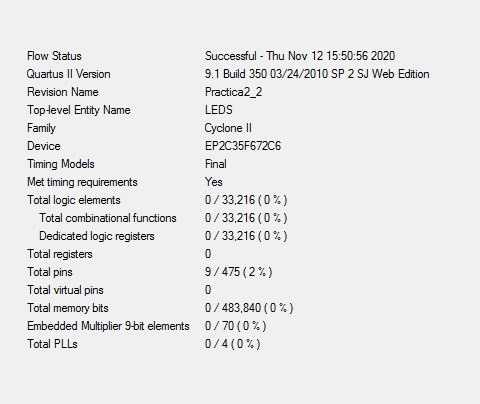
\includegraphics[width=130mm]{informeLEDS.jpeg}
		\end{center}
	\end{figure}
	
		\begin{table}[H]
		\centering
		 \begin{tabular}{|c | c|} 
			 \hline
			 Entrades & Descripció\\ [0.5ex] 
			 \hline
			 show & Marca si es mostren els leds verds o els vermells \\ [1ex] 
			 \hline\hline
			 Sortides & Descripció\\ [0.5ex] 
			 \hline
			 LED\_GREEN & Actiu si els leds verds shan d'encendre\\
			LED\_RED & Actiu si els leds vermells shan d'encendre\\ [1ex] 
			 \hline
		 \end{tabular}
	\end{table}
	
	
	\begin{figure}[H]
		\begin{center}
		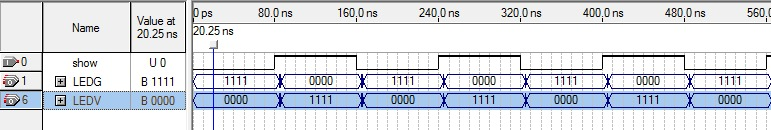
\includegraphics[width=130mm]{simulLEDS.jpeg}
		\end{center}
	\end{figure}
	
	Com es pot veure la simulació funcione en funció de la entrada show.
	\subsection{Programa principal}
	
	El programa principal ajunta tots els components mencionats anteriorment per tal de fer la part principal de la practica. El bloc keycode indica quin tipus de tecla es prem(AST, COI, BCD) es prem, que indica a control si ha de canviar d'estat o no. La entrada nkey marcarà si s'esta prement la tecla o no. Control decideixi si canviar el estat en funcio de la entrada com hem comentat abans. 
	
	La entrada keycode també s'envia a regs que actualitza o no els valors de opA i opB en funcio del estat actual. Aquests valors a la sortida es multipliquen en el multiplicador i el resultat s'envia a sel. En el cas que estiguem en el estat show treurà com a output el resultat, i en el cas que no hi siguem treura 11111111 cosa que farà que tots els llums del 7 bit quedin apagats.
	
	\begin{figure}[H]
		\begin{center}
		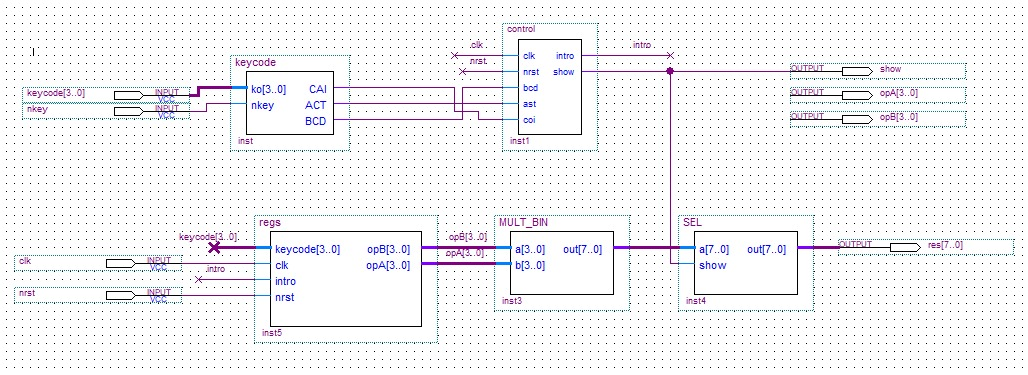
\includegraphics[width=130mm]{ppal.jpeg}
		\end{center}
	\end{figure}
	
	\begin{figure}[H]
		\begin{center}
		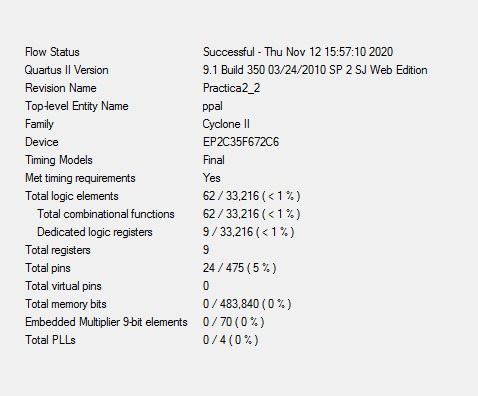
\includegraphics[width=130mm]{informePpal.jpeg}
		\end{center}
	\end{figure}
	
	\begin{table}[H]
		\centering
		 \begin{tabular}{|c | c|} 
			 \hline
			 Entrades & Descripció\\ [0.5ex] 
			 \hline
			 nkey(1) &  Marca si s'esta prement la tecla \\ 
			 keycode(4) & Marca la tecla que s'està prement \\
			 clk(1) & Es el rellotge que gestionara la memoria del sistema  \\
			 nrst(1) & Marcara si s'ha de resetejar a 0 o no \\ [1ex] 
			 \hline\hline
			 Sortides & Descripció\\ [0.5ex] 
			 \hline
			 show(1) & Diu si s'ha de mostrar la sortida o no\\ 
			 opA(8) & El valor del nombre A guardat a regs\\
			 opB(8) & El valor del nombre B guardat a regs\\
			 res(8) & Es el que s'ha de mostrar a la pantalla, la multiplicació o res\\ [1ex] 
			 \hline
		 \end{tabular}
	\end{table}
	
	\begin{figure}[H]
		\begin{center}
		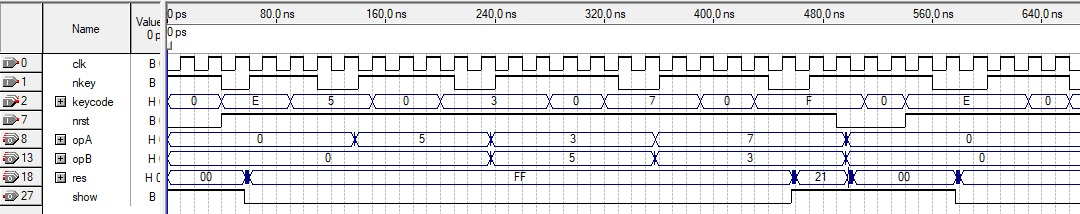
\includegraphics[width=130mm]{SimPpal.jpeg}
		\end{center}
	\end{figure}
	
	Per a veure si funcionava em simulat el seguent escenari. Primer hem entrat un coixinet per a passar al estat e insersio de dades st\_input. Hem entrat el 5 que ha actualitzat el valor de opA, i despres el 3 que ha actualitzat el valor de opB. En tot aquesta estona la sortida res ha estat apagada ja que el bit de show esta desactivat. Hem introduit despres la entrada 7 que ha mogut la 3 a opB i ha eliminat la 5. Despres d'aixo hem premut la tecla coixinet que ens ha deixat veure el resultat de la multiplicació. Despres d'això hem premut la tecla reset que ha posat tots els valors a 0 i el estat de control a st\_show, es a dir, amb el bit de show activat.
	
	\subsection{Final primera part}
	
	Despres de fer i testejar tots els components per separats i junts ho conectem tot a la placa de la forma que hem comentat al principi de la practica amb el següent cirquit, assignant a les entrades de la placa els pins que toqui per a que funcioni el diseny.
	
	\begin{figure}[H]
		\begin{center}
		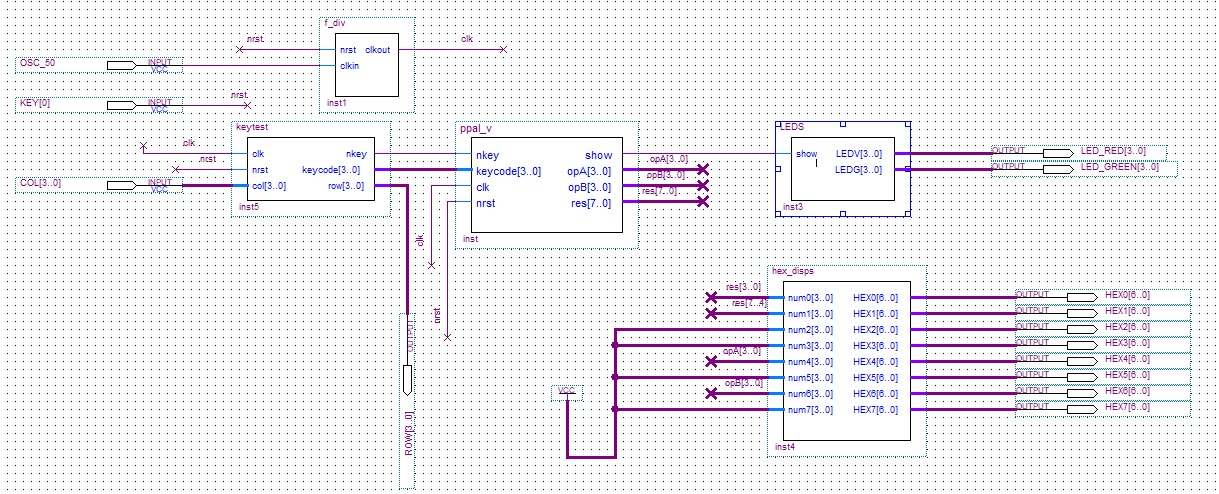
\includegraphics[width=130mm]{FinalDiseny.jpeg}
		\end{center}
	\end{figure}
	
	\begin{figure}[H]
		\begin{center}
		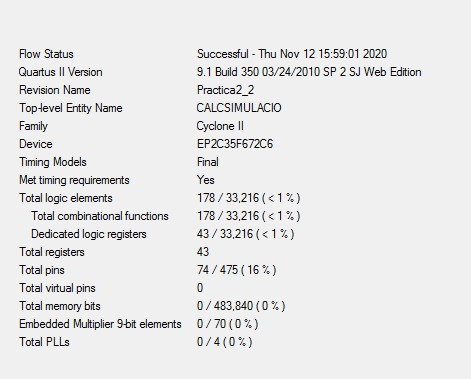
\includegraphics[width=130mm]{informeFINAL.jpeg}
		\end{center}
	\end{figure}
	
	\newpage
	
	\section{Part extra}
	
	Aquesta part hem realitzat els apartats a i c de la part extra. Per a fer aixo usarem el mateix diseny extern que el apartat anterior i per tant no el tornarem a explicar. L'unic que cambiem serà el programa principal junt amb tots els seus components que anirem explicant durant la memoria. Un petit resum es que per tal de saber si hem d'entrar A o B, dins de regs afegim 2 estats que ens ho indiquin. En el cas de que estiguem en la fase de introduir dades i haguem clicat A s'activara el estat de A. Per a la sortida(part c) calcularem totes les operacions demanades i amb un multiplexor seleccionarem la desitjada en funció de les tecles premudes durant el estat de show.
	
	\subsection{Keygroup actualitzat}
	
	Per tal de llegir, a mes dels nombres, lasterisc i el coixinet, les entrades A i B hem hagut d'afegir al codi VHDL dos sortides mes, A i B que diuen si la entrada keycode es refereix a aquestes tecles.
	\begin{lstlisting}[style=vhdl, frame=single, basicstyle=\tiny]
library ieee;
use ieee.std_logic_1164.all;

entity keycode_extra is
	port (nkey : in std_logic;
		  keycode : in std_logic_vector(3 downto 0);
		  bcd, ast, coi, A, B, C, D: out std_logic);
end keycode_extra;

architecture arq of keycode_extra is
begin
	bcd <= '1' when (nkey = '0' and (keycode = "0000" or
					 keycode = "0001" or
					 keycode = "0010" or
					 keycode = "0011" or
					 keycode = "0100" or
					 keycode = "0101" or
					 keycode = "0110" or
					 keycode = "0111" or
					 keycode = "1000" or
					 keycode = "1001"))
				else '0';
	ast <= '1' when nkey = '0' and keycode = "1110"
			   else '0';
	coi <= '1' when nkey = '0' and keycode = "1111"
			   else '0';
	A <= '1' when nkey = '0' and keycode = "1010"
			   else '0';
	B <= '1' when nkey = '0' and keycode = "1011"
			   else '0';
	C <= '1' when nkey = '0' and keycode = "1100"
			   else '0';
	D <= '1' when nkey = '0' and keycode = "1101"
			   else '0';
end arq;
\end{lstlisting}

\begin{figure}[H]
		\begin{center}
		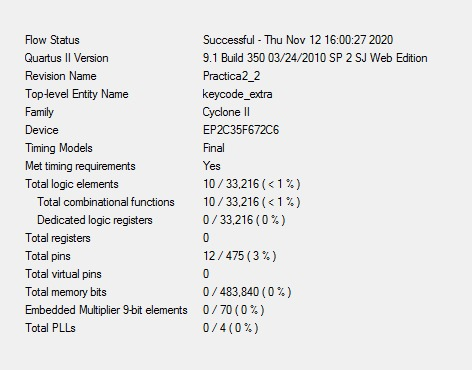
\includegraphics[width=130mm]{informekeygroupextra.jpeg}
		\end{center}
	\end{figure}

	\begin{figure}[H]
		\begin{center}
		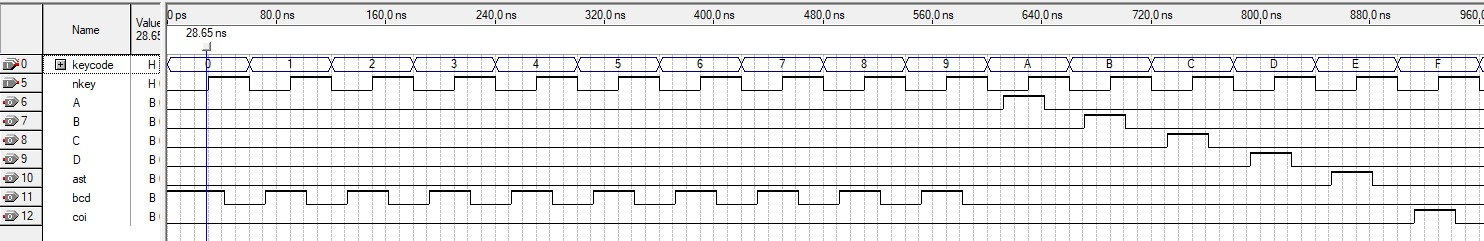
\includegraphics[width=130mm]{SimKCex.jpeg}
		\end{center}
	\end{figure}

	
	
	El component funciona ja que fa el mateix que el keygroup anterior amb la diferencia que quan la entrada en hexadecimal es A s'activa la sortida A i quan es B s'activa la B.
	
	\subsection{Regs actualitzat}
	
	Aquí caldrà afegir dos estats, el estat introA i introB, que indicaran si s'ha d'introduir A o B. Si la sortida A de keygroup està activada el estat passarà a ser introA, mentres que si es B passarà a ser introB. Si tant A com B son 0 es mantindrà igual. 
	
	Quan s'hagin d'introduir nombres ara, es mirarà en quin estat estem i si estem en el estat introA es canviarà el valor de A mentres que si estem en estat introB es canviarà B, sempre que el bit intro de la entrada estigui activat, ja que si no ho estigues, no s'haurien d'actualitzar els nombres ja que estariem en estat de show o la entrada seria asterisc o coixinet.
	
		\begin{lstlisting}[style=vhdl, frame=single, basicstyle=\tiny]
library ieee;
use ieee.std_logic_1164.all;

entity regs_extra2 is
	port(clk, nrst, intro, A, B : in std_logic;
		 keycode : in std_logic_vector(3 downto 0);
		 opA, opB: out std_logic_vector(3 downto 0));
end regs_extra2;

architecture arq of regs_extra2 is
type machine is ( entrA,  entrB);
signal aux1, aux2 : std_logic_vector(3 downto 0);
signal state : machine;
begin
process (clk, nrst)
begin 
	if nrst='0' then state <= entrA;
	end if;
	case state is
	    when entrA  => if B = '1' and (intro = '1')  then state <= entrB; 
	    end if;
	    when entrB  => if A = '1' and (intro = '1')  then state <= entrA; 
	    end if;
	end case;
	
	case state is
	    when entrA  =>  if(nrst = '0') 
			then aux1 <= "0000"; aux2 <= "0000";
		elsif(nrst='1') and (clk'event and clk = '1') and (intro = '1') 
			then aux1 <= keycode;
		end if;
	    when entrB  =>  if(nrst = '0') then aux1 <= "0000"; aux2 <= "0000";
		elsif(nrst='1') and (clk'event and clk = '1') and (intro = '1') then
			aux2 <= keycode;
		end if;
	end case;
end process;
opA <= aux1;
opB <= aux2;

end arq;
\end{lstlisting}

\begin{figure}[H]
		\begin{center}
		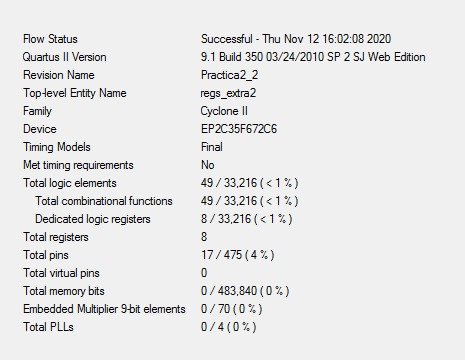
\includegraphics[width=130mm]{informeRegsextra.jpeg}
		\end{center}
	\end{figure}
	
	\begin{figure}[H]
		\begin{center}
		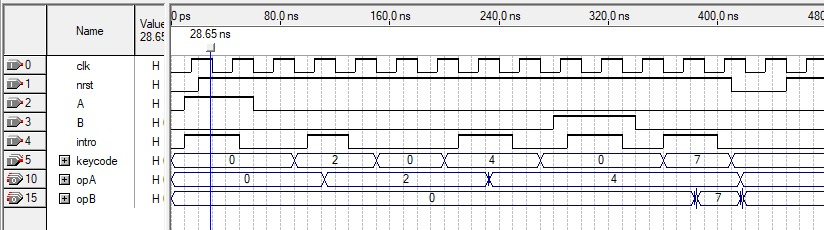
\includegraphics[width=130mm]{regsExtrSim.jpeg}
		\end{center}
	\end{figure}
	
	La simulacio es replica el seguent comportament. En primer lloc es prem la tecla A per a dir que les dades s'introduiran dins de A. S'introdueixen les dades 2 i 4, les dos sobre A. Despres es prem la tecla B que fa que es puguin introduir dades dins de B a on introduim el nombre 7 que es guarda a opB. Finalment cliquem el boto de reset que posa els valors de la sortida a 0.
	
	\subsection{Control actualitzat}
	
	Com que per tal de saber si hem d'actualitzar o no els estats de regs hem de saber si estem en el estat st\_intro o el estat st\_show, la sortida intro s'haura d'activar si estem a st\_intro i la entrada A o B estan activades. Per tant fem la següent modificació al codi.
	
			\begin{lstlisting}[style=vhdl, frame=single, basicstyle=\tiny]
library ieee;
use ieee.std_logic_1164.all;

entity Control_extra is
  port( clk, nrst, bcd, ast, coi, A, B, C, D : in std_logic;
		intro, show : out std_logic );
end Control_extra;

architecture arq of Control_extra is
  type machine is ( st_show,  st_intro);
  signal state : machine;
begin

  process(clk, nrst) 
  begin
	if nrst='0' then state <= st_show;
	elsif (clk'event and clk='1') then
		case state is
			when st_show  => if ast='1' then state <= st_intro; end if;
			when st_intro => if coi='1' then state <= st_show; 
							 else state <= st_intro;
							 end if;
		end case;
	end if;
end process;

intro <= '1' when state=st_intro and (bcd='1' or A = '1' or B = '1') else '0';
show  <= '1' when state=st_show else '0';

end arq;
\end{lstlisting}
	\begin{figure}[H]
		\begin{center}
		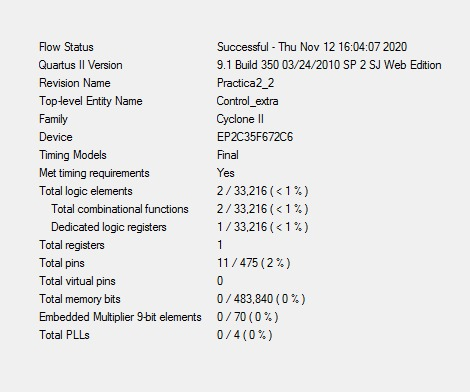
\includegraphics[width=130mm]{informeControlextra.jpeg}
		\end{center}
	\end{figure}

	\subsection{AperB actualitzat}
	
	En aquest modul cal afegir les funcionalitats de la part c extra que seran les de multiplicar A*A, B*B i la suma A+B. El component l'hem fet amb vhdl, pero com que el codi es molt llarg ja que cobrim molts casos i s'han de convertir totes les respostes a BCD. Per tant mostrarem una petita porcio del codi suficient per a entendre el funcionament.
	
				\begin{lstlisting}[style=vhdl, frame=single, basicstyle=\tiny]
library ieee;
use ieee.std_logic_1164.all;
use ieee.std_logic_unsigned.all;
use ieee.std_logic_arith.all;

entity AperB_extra is
	port(OpA, OpB : in std_logic_vector(3 downto 0);
		 AxB : out std_logic_vector(7 downto 0);
		 AxA : out std_logic_vector(7 downto 0);
		 BxB : out std_logic_vector(7 downto 0);
		 AmesB : out std_logic_vector(7 downto 0));
end AperB_extra;

architecture arq of AperB_extra is
signal OpA2, OpB2 : std_logic_vector(7 downto 0);
signal AxB_prov: std_logic_vector(7 downto 0);
signal AxA_prov : std_logic_vector(7 downto 0);
signal BxB_prov: std_logic_vector(7 downto 0);
signal AmesB_prov : std_logic_vector(7 downto 0);
begin
OpA2 <= "0000" & OpA;
OpB2 <= "0000" & OpB;
AxB_prov <= OpA*OpB;
AxA_prov <= OpA*OpA;
BxB_prov <= OpB*OpB;
AmesB_prov <= OpA2 + OpB2;

	with AxB_prov select AxB <=
		"10011001" WHEN "01010001" ,--81
		"01110010" WHEN "01001000" ,--72
		"01100100" WHEN "01000000" ,--64
		"01010110" WHEN "00111000" ,--56
		"01010100" WHEN "00110110" ,--54
		"01001001" WHEN "00110001" ,--49
		"01001000" WHEN "00110000" ,--48
		"01000101" WHEN "00101101" ,--45
					.
					.
					.
		"--------" WHEN OTHERS;
	
	with AxA_prov select AxA <=
		"10011001" WHEN "01010001" ,--81
		"01110010" WHEN "01001000" ,--72
		"01100100" WHEN "01000000" ,--64
		"01010110" WHEN "00111000" ,--56
		"01010100" WHEN "00110110" ,--54
		"01001001" WHEN "00110001" ,--49
		"01001000" WHEN "00110000" ,--48
		"01000101" WHEN "00101101" ,--45
					.
					.
					.
		"--------" WHEN OTHERS;
	
	with BxB_prov select BxB <=
		"10011001" WHEN "01010001" ,--81
		"01110010" WHEN "01001000" ,--72
		"01100100" WHEN "01000000" ,--64
		"01010110" WHEN "00111000" ,--56
		"01010100" WHEN "00110110" ,--54
		"01001001" WHEN "00110001" ,--49
		"01001000" WHEN "00110000" ,--48
		"01000101" WHEN "00101101" ,--45
					.
					.
					.
		"--------" WHEN OTHERS;
		
	with AmesB_prov select AmesB <=
		"00011000" when "00010010",--18
		"00010111" when "00010001",--17
		"00010110" when "00010000",--16
		"00010101" when "00001111",--15
		"00010100" when "00001110",--14
					.
					.
					.
		"--------" WHEN OTHERS;

end arq;
\end{lstlisting}

\begin{figure}[H]
		\begin{center}
		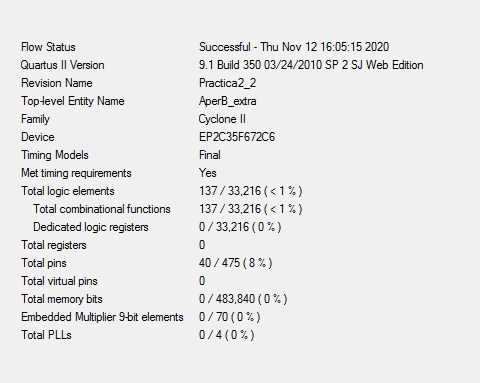
\includegraphics[width=130mm]{informeAperBextra.jpeg}
		\end{center}
	\end{figure}
	
	\begin{figure}[H]
		\begin{center}
		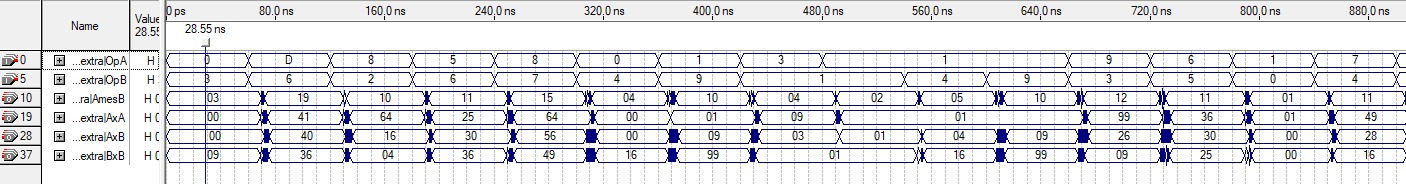
\includegraphics[width=130mm]{SimAxBextr.jpeg}
		\end{center}
	\end{figure}
	
	La simulacio mostra que els calculs s'efectuen correctament en tots els casos.
	
	\subsection{MUX de 4 entrades}
	Aquest component decidirà la sortida en funció de si introduim A, B, C o D a la placa durant la fase de show.
	
\begin{lstlisting}[style=vhdl, frame=single, basicstyle=\tiny]
library ieee;
use ieee.std_logic_1164.all;

entity MUX_extra is 
	port(A,B,C,D : in std_logic_vector(7 downto 0);
		sel : in std_logic_vector(3 downto 0);
		z: out std_logic_vector (7 downto 0));
end MUX_extra;

architecture arc of MUX_extra is
begin
	with sel select 
	z<= A when "1010",
		B when "1011",
		C when "1100",
		D when "1101",
		"11111111" when others;
end arc;
\end{lstlisting}

\begin{figure}[H]
		\begin{center}
		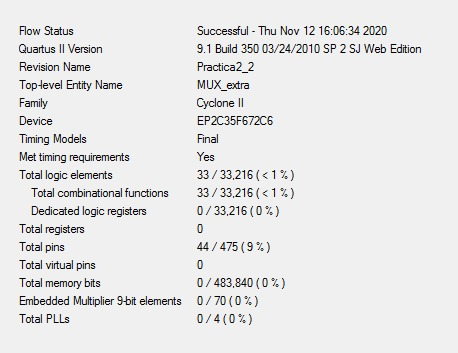
\includegraphics[width=130mm]{informeMUXextra.jpeg}
		\end{center}
	\end{figure}

	\begin{figure}[H]
		\begin{center}
		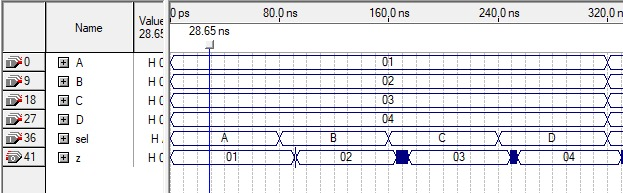
\includegraphics[width=130mm]{SimMUX.jpeg}
		\end{center}
	\end{figure}
	
	Podem veure que funciona ja que en funcio de la entrada sel ens mostra la entrada desitjada.
	
	\subsection{Programa principal extra}
	
	Aquest funciona molt semblant al de la part 1. Rep la tecla premuda que desxifra a trabes de keycode\_extra. Aquesta tecla la passa a control que actualitza les dades de estat i activa o no els bits de intro i show. 
	
	Per altra banda regs\_extra2 rep la informacio de la tecla premuda i de si es A o si es B, junt amb si control esta en el estat d'entrar dades o no ho esta. Si es A actualitza el estat de la mateixa manera que si es B. En el cas que que intro sigui 1 i keycode sigui un valor BCD s'actualitza la variable que toqui en funcio del estat. Aquestes dos sortides, opA i opB s'introdueixen dins de la calculadora que ens fa totes les operacions. A la sortida es conecta amb el multiplexor que en funció de la tecla premuda despres d'activar el bit show mostrara una cosa o altra. Finalment el bloc Sel decideix si mostrar o no la sortida en funcio de si esta activat el bit show o no.
	
	\begin{figure}[H]
		\begin{center}
		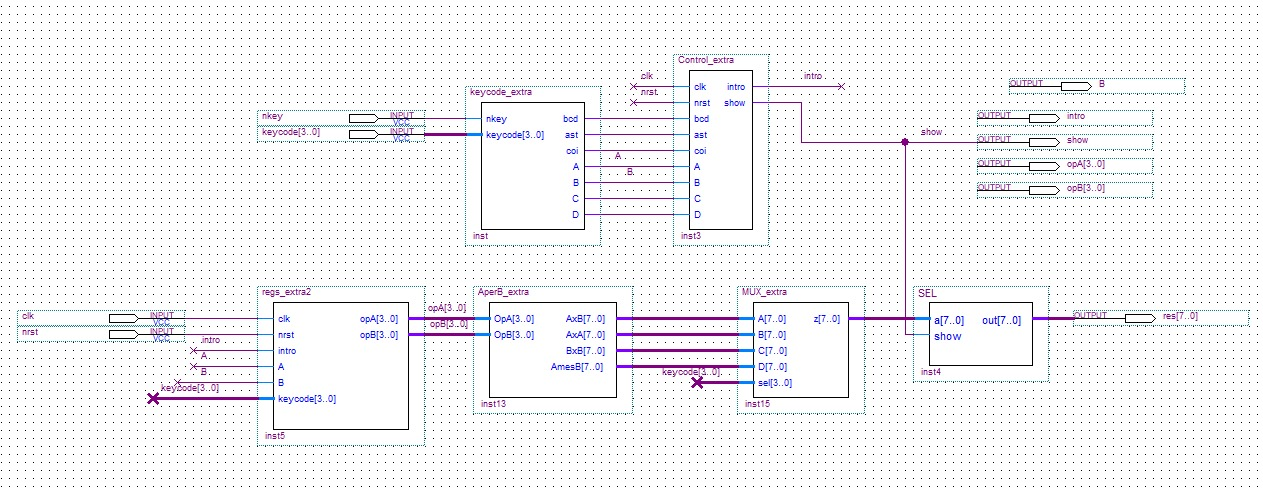
\includegraphics[width=130mm]{ppalExtra.jpeg}
		\end{center}
	\end{figure}
	
	\begin{figure}[H]
		\begin{center}
		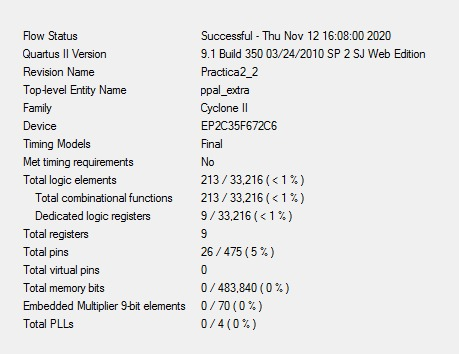
\includegraphics[width=130mm]{informePpalextra.jpeg}
		\end{center}
	\end{figure}
	
	\begin{figure}[H]
		\begin{center}
		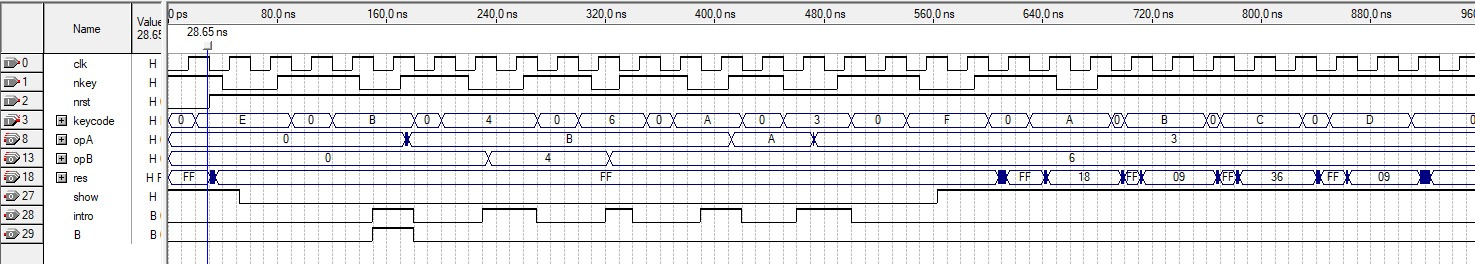
\includegraphics[width=130mm]{SimPpalExtra.jpeg}
		\end{center}
	\end{figure}
	
	Per veure si funcionava hem simulat les seguents entrades. Primer introduim un asterisc per a marcar l'inici de les entrades. Despres marquem que volem entrar els valors de B, que introduim el nombre 4 i despres el 6. Despres indiquem que volem introduir els nombres dins de A, al qual introduim el nombre 3. Despres clicant coixinet activem el bit de show. Clicant A ens mostra A*B, clicant B ens mostra A*A, clicant C ens mostra B*B i clicant D ens mostra A+B. Per tant el diseny funciona a la perfecció.
	
	

\section{Part extra 2}

Aquesta part cobreix la explicacio de la part b del extra. Tot i que tenim una idea de com es fa, no hem tingut temps de debuguejar tot el codi i simularho. Tot i així mostrarem els components casi complets i com seria el seu funcionament en el cas de que estiguessin construits bé.

\subsection{Regs actualitzat}

Per tal de saber si s'entrarà un nombre positiu o negatiu hem afegit dos nous estats, entrAmenys i entrBmenys. Aquest gestionaran la entrada en el cas que sigui negativa. Si estem en aquest estat i s'entra una dada, s'aplicarà una conversió de BCD a CA2 i es treurà el resultat. El codi seria semblant al seguent.

\begin{lstlisting}[style=vhdl, frame=single, basicstyle=\tiny]
library ieee;
use ieee.std_logic_1164.all;
USE IEEE.NUMERIC_STD.ALL;

entity regs_extra3 is
	port(clk, nrst, intro, A, B, C : in std_logic;
		 keycode : in std_logic_vector(3 downto 0);
		 opA, opB: out std_logic_vector(3 downto 0));
end regs_extra3;

architecture arq of regs_extra3 is
type machine is ( entrAmes,  entrBmes, entrAmenys,  entrBmenys);
signal aux1, aux2  : std_logic_vector(3 downto 0);
signal state : machine;
begin
process (clk, nrst)
begin 
	if nrst='0' then state <= entrAmes;
	end if;
	case state is
		when entrAmes  => if B = '1' and (intro = '1') then state <= entrBmes; 
				elsif C = '1' and (intro = '1') then state <= entrAmenys; 
				end if;			  
		when entrBmes  => if A = '1' and (intro = '1') then state <= entrAmes; 
				elsif C = '1' and (intro = '1') then state <= entrBmenys; 
				end if;
		when entrAmenys  => if B = '1' and (intro = '1') then state <= entrBmes; 
				elsif A = '1' and (intro = '1') then state <= entrAmes; 
				end if;	
		when entrBmenys  => if A = '1' and (intro = '1') then state <= entrAmes; 
				elsif B = '1' and (intro = '1') then state <= entrBmes;
				end if;		
	end case;
	
	case state is
		when entrAmes  =>  if(nrst = '0') then aux1 <= "0000"; 
									 aux2 <= "0000";
					 elsif(nrst='1') and (intro = '1') then
							aux1 <= keycode;
							end if;
		when entrBmes  =>  if(nrst = '0')  then aux1 <= "0000"; 
									  aux2 <= "0000";
					elsif ((nrst='1')  and (intro = '1')) then
							aux2 <= keycode;
						end if;
		when entrAmenys  =>  if(nrst = '0')then aux1 <= "0000"; 
								aux2 <= "0000";
					elsif(nrst='1')  and (intro = '1') then
						aux1 <= (Aqui aniria keycode en CA2);
						end if;
		when entrBmenys  =>  if(nrst = '0') then aux1 <= "0000"; 
								aux2 <= "0000";
					elsif(nrst='1') and (intro = '1') then
						aux2(0) <= (Aqui aniria keycode en CA2);
						end if;
	end case;
end process;
opA <= aux1;
opB <= aux2;

end arq;
\end{lstlisting}

\subsection{AperB actualitzat}

Aquest component caldrà actualitzarlo per tal de fer les operacions en signed decimal. El codi sera el mateix, però canviaran les seguents linees.

\begin{lstlisting}[style=vhdl, frame=single, basicstyle=\tiny]
USE IEEE.NUMERIC_STD.ALL;
		.
		.
		.
AxB_prov <= signed(OpA)*signed(OpB);
AxA_prov <= OpA*OpA;
BxB_prov <= OpB*OpB;
AmesB_prov <= signed(OpA2) + signed(OpB2);
\end{lstlisting}

\subsection{Signe 7s}
	Finalment per afegir el signe hem fet una descripció vhdl del modul Signe 7s i amb el modul de Signe 7s i a partir dels interuptors SW i una porta XOR aconseguim el resultat desitjat. Hem posat una entrada num i una altra entrada show de tal manera que quan introduirem numeros per teclat el signe estigui apagat .

	\begin{lstlisting}[style=vhdl, frame=single, basicstyle=\tiny]
library ieee;
use ieee.std_logic_1164.all;

entity Signe_7s is 
	port(num, show : in std_logic;
		HEX : out std_logic_vector(6 downto 0));
		
end Signe_7s ;

architecture tdv of Signe_7s is
begin

HEX <= "0111111" when (num = '1' and show = '1') else "1111111";
end tdv;
\end{lstlisting}

\begin{figure}[H]
		\begin{center}
		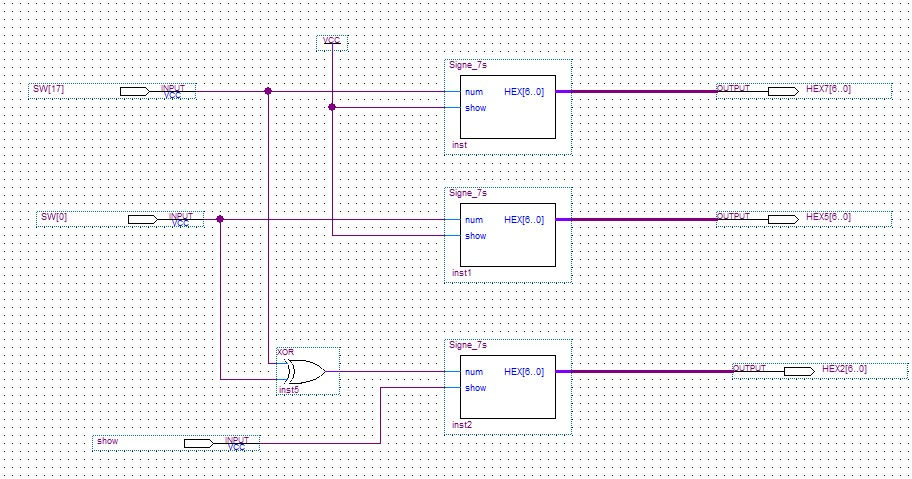
\includegraphics[width=130mm]{signeextra.jpeg}
		\end{center}
	\end{figure}
	\begin{figure}[H]
		\begin{center}
		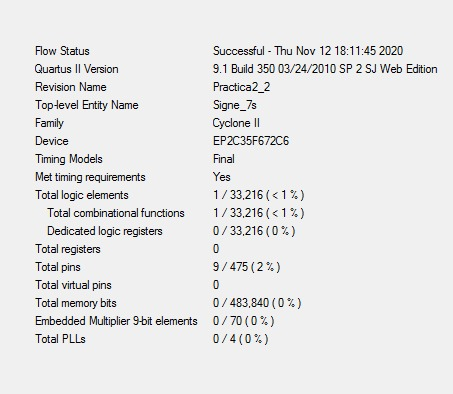
\includegraphics[width=130mm]{informeSigne.jpeg}
		\end{center}
	\end{figure}
\end{document}


